\chapter{Experimental Results}
\label{ch:experiments}

\section{Experimental Design}

For this project, my experimental design revolves around the fact that we are bypassing
a login screen and with that, being able to gain access to a large quantity of data that
consists of variables such as firstname, lastname, age, salary, eye color, ethnicity
as well as a few other factors. The way that the experiment had been set up was by first
researching a lot about the topic. SQL injection is a very popular injection technique
so there is a lot of documentation out there on the subject. Another big point was figuring out how to exactly inject the SQL code to
bypass the log-in. While initially thinking about this, it had sounded much more
complicated, but once we had researched and planned out what needed to happen, things
started coming together. The experiment here was seeing if not only could it be possible to create a database and web application but bypass
the login with just some SQL query statements. From the introduction, there was talk about
the different possible SQL query statements that are common to try and bypass a login
that is associated with web applications. Since we are trying to figure out why this
might have been the case though, and we thought that it would be best to try and look at the code to try and figure out
why this might be the case. So for here, the starting point would be the SQL
query statement that is used to connect the web application and the database. For this
particular project, one would not only have to come up with a query statement that will connect
the two but also come up with a piece of code that one can inject into my SQL query statement.
Let us start one step at a time though. To connect the database and the web application
with the query statement, one would have to give it the parameters that are necessary so it will choose
the right table, and display all of the information that is desired if it has the proper
login credentials. If it doesn't then it will just redirect to a different page. With this
knowledge, we now must figure out the best query statement to connect the two. This
is what we came up with.


\bigskip
\bigskip
\begin{lstlisting}
cur = g.db.execute("select username from managers where username=\""+request.form['username']+"\""+"and password=\""+request.form['password']+"\"")
\end{lstlisting}
\bigskip
\bigskip


\section{Evaluation}

Based on this query, and the SQL injection piece of code that had been shown earlier, we
can bypass the login and see all of the important data. Everything
that is in the database will also be displayed to us. One could say based on us being
able to do that, The evaluation of my experiment went pretty well. We had predicted
that one could bypass the log-in if the user knew what the SQL query statement was and since
we created it, we of course knew what it was. These are the results below. As you can see the id for web application and for the database are the same meaning the database associated with each is the same, the difference is how each were accessed.

\bigskip
\bigskip
\begin{figure}[hbt!]
\centering
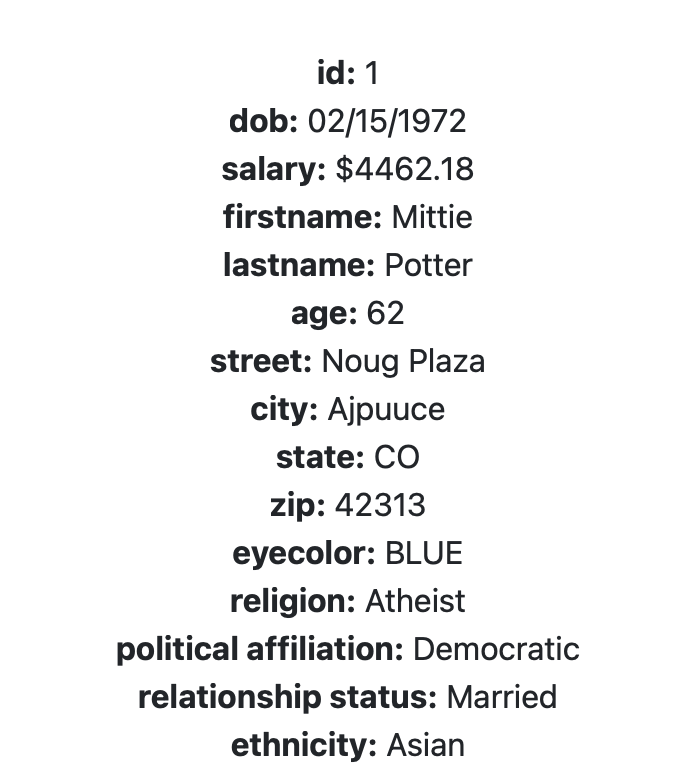
\includegraphics[height=3in]{../images/access-1.png}%
\caption{Data on Website}
\label{fig:data on website}
\end{figure}
\bigskip

\bigskip
\begin{figure}[hbt!]
\centering
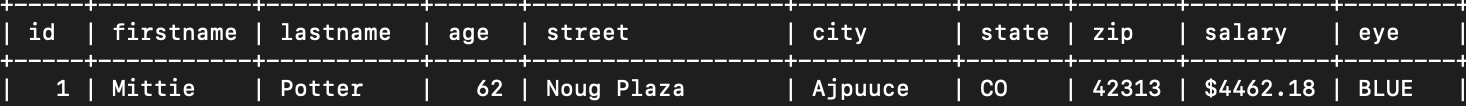
\includegraphics[width=6in]{../images/access-2.png}%
\caption{Data in Terminal}
\label{fig:data in terminal}
\end{figure}
\bigskip
\bigskip



\section{Threats to Validity}

There could be arguments with the validity of my work. One could argue
that for my SQL injection code, I made it so that whatever was had put in the username
column would be in the username column in my database. Ultimately making it just
log me in instead of bypassing the login. Another argument could be that
I didn't create the VPN and database cluster together, meaning that you don't necessarily have to connect to the VPN to connect to the database. This of course
though, is false. Certain trusted servers allow the database to be logged
into from. The way that I had set it up is that you have to be connected
to a specific server to be able to log in, and in my case, it is the server
that we are connected to through our VPN. There may be more claims as to what are
other threats to validity, but with the work that I have done and everything I was
able to complete, I believe my work stands solid. A big point for validity though is the notion
that an SQLite database was used to store the data that is associated with the web application. This could be considered a threat because SQLite databases are not as robust as industry-standard ones such as MySQL and PostgreSQL. The industry-standard ones have better security so by-passing a log in the way that was demonstrated wouldn't be as easy as it seems. The idea though is still the same. MySQL is not the end-all-be-all-perfect database that has no security issues so my point still stands solid. Security associated with web applications and databases needs to be improved upon and better.